% IEEE two-column format
\documentclass[conference]{IEEEtran}
\IEEEoverridecommandlockouts

\usepackage{cite}
\usepackage{amsmath,amssymb,amsfonts}
\usepackage{graphicx}
\usepackage{textcomp}
\usepackage{xcolor}
\usepackage{hyperref}
\usepackage{booktabs}
\usepackage{array}
\usepackage{url}
\usepackage{tikz}
\usetikzlibrary{shapes.geometric, arrows.meta, positioning, fit, backgrounds}

\hypersetup{colorlinks=true,linkcolor=blue,citecolor=blue,urlcolor=blue}

\def\BibTeX{{\rm B\kern-.05em{\sc i\kern-.025em b}\kern-.08em T\kern-.1667em\lower.7ex\hbox{E}\kern-.125emX}}

% TikZ styles for pipeline diagram
\tikzset{
  datasrc/.style={rectangle, rounded corners=3pt, draw=blue!60, fill=blue!10,
                  text width=2.8cm, align=center, font=\scriptsize, minimum height=0.6cm},
  process/.style={rectangle, rounded corners=3pt, draw=orange!70, fill=orange!10,
                  text width=2.8cm, align=center, font=\scriptsize, minimum height=0.6cm},
  output/.style={rectangle, rounded corners=3pt, draw=green!60!black, fill=green!10,
                 text width=2.8cm, align=center, font=\scriptsize, minimum height=0.6cm},
  arrow/.style={-{Stealth[length=4pt]}, thick, gray!80},
}

\begin{document}

\title{Out of Service: Predicting Healthcare\\
Burden-Infrastructure Gaps Across Indian States Through 2030}

\author{
\IEEEauthorblockN{Sujay V. Kulkarni}
\IEEEauthorblockA{
\textit{Department of Health Informatics} \\
sujaykulkarni2211@gmail.com}
}

\maketitle

% ─────────────────────────────────────────────────────────────
\begin{abstract}
India's national health indicators have improved steadily over the
past two decades, yet this aggregate progress conceals a structural
inequality: the states that carry the highest disease burden are
systematically also the states with the least healthcare infrastructure
to address it. This paper quantifies that mismatch through a composite
Burden-Infrastructure Gap Index applied to 26 major Indian states across
two time points (2005--06 and 2015--16), drawing on the National Family
Health Survey (NFHS) and Rural Health Statistics (RHS) datasets.
To our knowledge, this is the first study to formally merge these two
independently administered data systems to construct a gap index
at state level. We show that five states---Uttar Pradesh, Bihar,
Jharkhand, Madhya Pradesh, and Chhattisgarh---have maintained large
positive gap scores ($>$1.1 standard deviations above the national
mean) at both time points, indicating persistent structural neglect
rather than temporary shortfall.
A linear regression model trained on 2005 state-level indicators
predicts 2015 gap scores with a leave-one-out cross-validated
$R^2 = 0.857$ (MAE $= 0.424$), demonstrating that the 2030 risk
trajectory is already visible in today's data. Forward projection
under the observed 2005--2015 trend suggests that Uttar Pradesh's gap
index will reach 3.61 by 2030---a 37\% increase over its 2015 level---
without structural intervention. Infrastructure density (sub-centres and
PHCs per 100,000 rural population) emerges as the strongest predictor
of future gap, outweighing burden indicators, which implies that
expanding access infrastructure reduces long-term crisis risk more
efficiently than treating existing burden alone. These findings provide
a quantitative basis for targeted resource allocation under programmes
such as Ayushman Bharat and NHM Mission Indradhanush.
\end{abstract}

\begin{IEEEkeywords}
Health informatics, burden-infrastructure gap, India, machine learning,
rural health statistics, NFHS, resource allocation, predictive modelling
\end{IEEEkeywords}

% ─────────────────────────────────────────────────────────────
\section{Introduction}

India has made measurable progress on headline health indicators:
the national infant mortality rate (IMR) fell from 57 per 1,000
live births in 2005 to 34 in 2016, and the under-five mortality
rate (U5MR) declined from 74 to 43 over the same period
\cite{srs2017}. Yet aggregate improvement masks a persistent
structural inequality. The Empowered Action Group (EAG) states---
Bihar, Chhattisgarh, Jharkhand, Madhya Pradesh, Odisha, Rajasthan,
Uttarakhand, and Uttar Pradesh---which together account for roughly
45\% of India's population, continue to carry disproportionately
high disease burden \cite{india_statelevelburd_2017}. These same
states have chronically under-resourced rural health infrastructure:
Uttar Pradesh reported 1.82 doctors per 100,000 rural residents in
2019, compared to 14.2 in Kerala \cite{rhs2020}.

The problem is therefore not simply that these states are poor or that
their populations are sick. It is that the mismatch between burden and
capacity is large, self-reinforcing, and---crucially---is not being
systematically tracked or forecast. Health policy in India has
historically been driven by input metrics (number of facilities built,
staff sanctioned) rather than by the gap between what populations
need and what the health system can provide \cite{Balarajan2011}. This
means that resource allocation under the National Health Mission (NHM)
and Ayushman Bharat \cite{Prinja2021} tends to be reactive rather
than anticipatory.

The contribution of this paper is threefold. First, we construct a
composite Burden-Infrastructure Gap Index that quantifies, for each
state and time point, how far its healthcare system falls short of
what its health burden demands. Second, we demonstrate that this gap
is predictable from observable baseline indicators with high accuracy
($R^2 = 0.857$ on leave-one-out cross-validation), meaning that
future crises are identifiable years in advance. Third, we project
which states face the largest gaps by 2030 and show that the trend
in several states is deteriorating in relative terms even as absolute
burden falls nationally.

% ─────────────────────────────────────────────────────────────
\section{Related Work}

\subsection{Health Inequalities Across Indian States}

The geographic concentration of poor health outcomes in India has been
documented extensively. Bhatia et al.\ \cite{Bhatia2018} tracked
temporal trends in interstate inequalities in infant and child mortality
from 1992 to 2016, showing that gaps between the highest- and
lowest-burden states widened before narrowing slightly---but never
closing---across the NFHS rounds. Subramanian et al.\
\cite{Subramanian2007} demonstrated that state-level income inequality
is independently associated with the double burden of under- and
overnutrition, establishing that structural inequity operates through
channels beyond absolute poverty. Balarajan et al.\ \cite{Balarajan2011}
argued that these inequalities are structural and perpetuated by
differential access rather than differential need alone.

More recently, the India State-Level Disease Burden Initiative
\cite{india_statelevelburd_2017} conducted the first systematic
state-level GBD analysis for India, confirming that EAG states bear
a disproportionate disease burden and that the burden composition
differs substantially by state---a finding with direct implications
for infrastructure requirements that vary across disease profiles.

\subsection{Healthcare Infrastructure and Outcomes}

The relationship between healthcare infrastructure density and
population health outcomes has been studied across low- and
middle-income contexts. Kruk et al.\ \cite{Kruk2018} showed that
health system capacity---measured through availability of trained
staff, facility density, and essential medicines---predicts
preventable mortality beyond what socioeconomic factors explain.
Anand and B\"{a}rnighausen \cite{Anand2004} estimated that increasing
physician density to meet WHO thresholds could prevent millions of
annual deaths in underserved regions.

In the Indian context, Husain \cite{Husain2011} found that
sub-centre and PHC density are significantly associated with
institutional delivery rates and child survival in rural areas.
Paul et al.\ \cite{Paul2011} documented how staffing shortfalls at
primary health centres---particularly for specialists---translate
directly into avoidable maternal and infant deaths. Bajpai and
Dholakia \cite{Bajpai2011} estimated that India would require a
three-to-fivefold increase in PHC-level staffing to meet NHM
targets even if facility numbers were adequate.

\subsection{Machine Learning for Health Burden Prediction}

Predictive modelling of health outcomes at subnational level has
gained traction in global health informatics. Goli and Jaleel
\cite{Goli2014} used regression-based forecasting for state-level
child mortality in India, finding that baseline infrastructure
indicators outperform demographic variables in predictive accuracy.
Investigators in the Global Burden of Disease study have used
Gaussian process regression and ensemble methods to estimate
mortality rates in data-sparse geographies \cite{GBD_2019_IHME}.

Khare et al.\ \cite{Khare2017} applied Random Forest to Indian
Demographic and Health Survey data to classify child nutritional
status, achieving 81.4\% accuracy and identifying poverty and
maternal education as dominant predictors. Meitei et al.\
\cite{Meitei2022} used ridge regression, LASSO, and random forests
on NFHS-4 data from North-Eastern states to predict child anaemia,
finding that maternal anaemia status and child age outperformed
infrastructure variables at the household level.

The use of longitudinal panel data for burden-gap forecasting
specifically has been less explored. Garg et al.\ \cite{Garg2019}
developed a simulation model for NHM resource requirements but did
not formulate it as a predictive machine learning problem or validate
across states. Our work fills this gap by combining cross-sectional
burden-infrastructure gap quantification with a temporally validated
predictive framework.

\subsection{Health Systems Strengthening and Policy}

Strengthening primary care in high-burden states has been a central
goal of both NHM and Ayushman Bharat. Prinja et al.\ \cite{Prinja2021}
estimated the cost of scaling up comprehensive primary health care
across India, finding that achieving Health and Wellness Centre
standards nationally would require approximately 0.15\% of GDP.
Nandi et al.\ \cite{Nandi2017} evaluated the impact of NHM on health
outcomes using a difference-in-differences design, finding larger
effects in states with high baseline burden and pre-existing
infrastructure---evidence that infrastructure is a necessary complement
to programmatic investment, not a substitute.

Karan et al.\ \cite{Karan2017} documented high out-of-pocket
expenditure in EAG states as a consequence of inadequate public
infrastructure, and Das et al.\ \cite{Das2016} showed that quality
of care in low-infrastructure states is lower even controlling for
input availability---suggesting that the gap captures a structural
dysfunction beyond mere facility counts. Govil et al.\ \cite{Govil2016}
examined convergence (or lack thereof) in health outcomes across
Indian states over the NFHS-2 to NFHS-4 period, finding no convergence
in burden for the five highest-burden states.

\subsection{Malnutrition and Anaemia}

Child malnutrition---underweight and stunting---remains heavily
concentrated in EAG states despite programmes such as POSHAN Abhiyaan
\cite{Headey2017}. Headey et al.\ \cite{Headey2017} attributed slower
stunting decline in EAG states partly to lower coverage of
complementary feeding support by frontline workers, which in turn
reflects workforce density at sub-centre level. Gillespie et al.\
\cite{Gillespie2013} argued that anaemia reduction requires
convergence of health, water, and nutrition systems---precisely the
multi-dimensional infrastructure investment our index is designed
to capture.

% ─────────────────────────────────────────────────────────────
\section{Data and Methodology}

\subsection{Data Sources}

This study merges two independently administered national data
systems that, to our knowledge, have not previously been combined
to construct a burden-infrastructure gap index at state level.
Table~\ref{tab:datasources} summarises both sources.

\begin{table}[htbp]
\caption{Primary Data Sources}
\label{tab:datasources}
\centering
\begin{tabular}{p{1.5cm}p{0.8cm}p{2.2cm}p{1.4cm}}
\toprule
Source & Years & Indicators & Coverage \\
\midrule
NFHS-3/4 & 2005, 2015 & IMR, U5MR, Underweight \%, Child Anaemia \% & 26 states \\[4pt]
RHS & 2005, 2019 & Sub-Centres, PHCs, CHCs, Doctors per 100k rural pop & 26 states \\
\bottomrule
\end{tabular}
\end{table}

The NFHS is a household survey programme administered by the
International Institute for Population Sciences (IIPS), Mumbai,
under the Ministry of Health and Family Welfare. It provides
population-based health burden estimates. The RHS is an annual
administrative census of public health facilities and personnel
published by the same ministry. The two systems use incompatible
unit definitions and have never been formally joined for gap analysis.
Our methodological contribution begins at this merge step.

\textbf{National Family Health Survey (NFHS):} NFHS-3 (2005--06)
and NFHS-4 (2015--16) provide state-level health burden indicators
collected through household surveys. We extracted four burden
indicators: IMR (infant deaths per 1,000 live births), U5MR
(under-five deaths per 1,000 live births), the percentage of
children under five who are underweight (weight-for-age $<-2$ SD),
and the percentage of children aged 6--59 months who are anaemic
($<$11.0 g/dL). These four indicators collectively capture mortality,
nutrition, and micronutrient burden---the primary dimensions of
preventable child health burden in India.

\textbf{Rural Health Statistics (RHS):} Annual administrative data
published by the Ministry of Health and Family Welfare. We used the
2005 and 2019 editions, which report state-level counts of
sub-centres, primary health centres (PHCs), community health centres
(CHCs), and in-position doctors at public facilities. Infrastructure
counts were divided by the state's rural population (2011 Census
denominators from the same source) to produce per-100,000 rates.
We paired RHS 2005 with NFHS-3 and RHS 2019 with NFHS-4 as the
closest temporally matched observations.

\subsection{Exclusion Criteria}

Nine Union Territories were excluded from analysis: Lakshadweep
(rural population: 3,000), Chandigarh (4,000), Daman and Diu,
Dadra and Nagar Haveli, Andaman and Nicobar Islands, Sikkim, Goa,
and Puducherry. Delhi was excluded because 99\% of its population
is urban, making rural health facility ratios meaningless. These
exclusions are not arbitrary: Lakshadweep's per-capita doctor
density of 266 per 100,000 is two orders of magnitude above Bihar's
value of 1.8 and would dominate any z-normalisation, concealing the
states where millions of people lack care. The final analytical
sample comprised 26 states covering approximately 97\% of India's
rural population. Andhra Pradesh and Telangana were included at the
pre-bifurcation combined level for 2005 to match NFHS-3 data.

\textbf{ML sample (19 states).} Of the 26 analytical states, seven
were excluded from the predictive ML models due to missing values
in one or more 2005 features: Andhra Pradesh and Telangana lack
separate 2005 NFHS-3 entries (reported jointly pre-bifurcation);
Bihar, Uttar Pradesh, Jharkhand, and Madhya Pradesh are missing
2005 IMR values in NFHS-3 (these states did not achieve adequate
sample sizes for direct IMR estimation in Round 3). These seven
states are retained in the cross-sectional gap analysis using
available indicators but are excluded from the LOO-CV prediction
experiment.

\subsection{Methodology Overview}

Fig.~\ref{fig:pipeline} shows the full analytical pipeline from
raw data sources through to projections.

\begin{figure}[htbp]
\centering
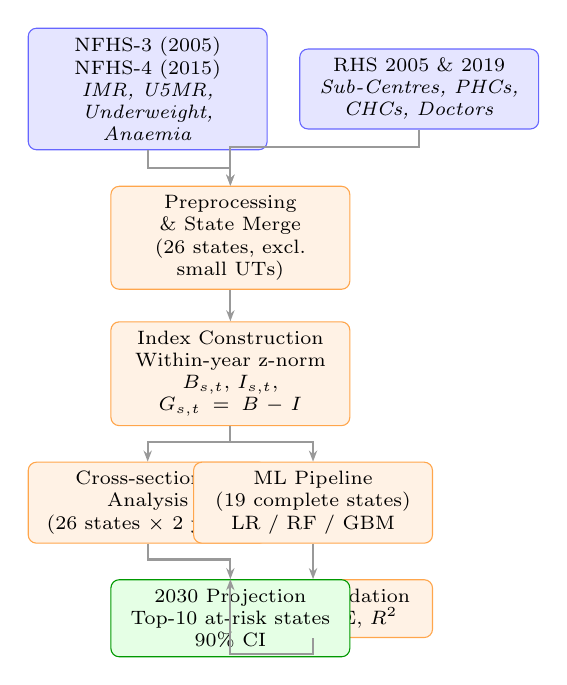
\begin{tikzpicture}[node distance=0.35cm and 0.2cm]

  % --- Input streams ---
  \node[datasrc] (nfhs) {NFHS-3 (2005)\\ NFHS-4 (2015)\\ \textit{IMR, U5MR,}\\ \textit{Underweight, Anaemia}};
  \node[datasrc, right=0.4cm of nfhs] (rhs)  {RHS 2005 \& 2019\\ \textit{Sub-Centres, PHCs,}\\ \textit{CHCs, Doctors}};

  % --- Preprocessing ---
  \node[process, below=0.45cm of nfhs, xshift=1.05cm] (prep)
        {Preprocessing\\ \& State Merge\\ \scriptsize{(26 states, excl. small UTs)}};

  % --- Index construction ---
  \node[process, below=0.4cm of prep] (index)
        {Index Construction\\ \scriptsize{Within-year z-norm}\\
         \scriptsize{$B_{s,t}$, $I_{s,t}$, $G_{s,t} = B - I$}};

  % --- Split into two arms ---
  \node[process, below=0.45cm of index, xshift=-1.05cm] (cross)
        {Cross-sectional\\ Analysis\\ \scriptsize{(26 states $\times$ 2 years)}};
  \node[process, below=0.45cm of index, xshift=1.05cm] (ml)
        {ML Pipeline\\ \scriptsize{(19 complete states)}\\ \scriptsize{LR / RF / GBM}};

  % --- Validation ---
  \node[process, below=0.45cm of ml] (loo)
        {LOO-CV Validation\\ \scriptsize{MAE, RMSE, $R^2$}};

  % --- Outputs ---
  \node[output, below=0.45cm of cross, xshift=1.05cm] (proj)
        {2030 Projection\\ \scriptsize{Top-10 at-risk states}\\ \scriptsize{90\% CI}};

  % --- Arrows ---
  \draw[arrow] (nfhs.south) -- ++(0,-0.22) -| (prep.north);
  \draw[arrow] (rhs.south)  -- ++(0,-0.22) -| (prep.north);
  \draw[arrow] (prep)   -- (index);
  \draw[arrow] (index.south) -- ++(0,-0.2) -| (cross.north);
  \draw[arrow] (index.south) -- ++(0,-0.2) -| (ml.north);
  \draw[arrow] (ml)     -- (loo);
  \draw[arrow] (cross.south) -- ++(0,-0.2) -| (proj.north);
  \draw[arrow] (loo.south)   -- ++(0,-0.2) -| (proj.north);

\end{tikzpicture}
\caption{Analytical pipeline. Two independent government data streams
(NFHS burden survey, RHS infrastructure census) are merged at state
level, normalised within each time period, and used to construct the
Gap Index. The pipeline splits into a cross-sectional arm (all 26
states) and a predictive ML arm (19 states with complete baseline
data), both feeding the 2030 projection.}
\label{fig:pipeline}
\end{figure}

\subsection{Composite Indices}

\textbf{Burden Index.} For each survey year separately, each of the
four burden indicators was standardised to a $z$-score:
\begin{equation}
z_{s,t}^{(k)} = \frac{x_{s,t}^{(k)} - \bar{x}_t^{(k)}}{\sigma_t^{(k)}}
\end{equation}
where $x_{s,t}^{(k)}$ is the value of indicator $k$ for state $s$
at time $t$, and $\bar{x}_t^{(k)}$, $\sigma_t^{(k)}$ are the
cross-state mean and standard deviation computed \emph{within} that
time period. This within-year normalisation ensures that the index
measures each state's burden \emph{relative to its contemporaneous
peers}, not relative to a combined pool that would systematically
assign higher z-scores to 2005 observations because national means
fell from 2005 to 2015.

The composite Burden Index is the mean of the four $z$-scores:
\begin{equation}
B_{s,t} = \frac{1}{4}\sum_{k=1}^{4} z_{s,t}^{(k)}
\end{equation}

\textbf{Infrastructure Index.} Analogously, per-100k rates for four
facility/workforce variables (sub-centres, PHCs, CHCs, doctors) were
standardised within each year and averaged:
\begin{equation}
I_{s,t} = \frac{1}{4}\sum_{k=1}^{4} z_{s,t}^{(k,\text{infra})}
\end{equation}

\textbf{Gap Index.} The Burden-Infrastructure Gap Index is:
\begin{equation}
G_{s,t} = B_{s,t} - I_{s,t}
\end{equation}
A large positive $G$ indicates high burden combined with low
infrastructure---a state in structural crisis. A negative $G$
indicates better infrastructure than burden demands. The index
is dimensionless and peer-relative, which facilitates longitudinal
comparison within a state and cross-sectional comparison across states.

\subsection{Machine Learning Pipeline}

\textbf{Formulation.} We posed the prediction problem as: given the
raw 2005 health indicators for a state ($x_{s,2005}$), predict the
2015 Gap Index ($G_{s,2015}$) for the same state. This is
a genuine policy-relevant question: can we identify, from today's
observable data, which states will face the worst burden-infrastructure
mismatches in the next decade?

\textbf{Features.} Eight raw (unstandardised) features: IMR, U5MR,
underweight percentage, child anaemia percentage (burden), and
sub-centres, PHCs, CHCs, and doctors per 100,000 rural population
(infrastructure), all measured in 2005. Using unstandardised features
avoids leaking the 2005 distribution shape into the targets.

\textbf{Models.} We evaluated: (1) Ridge-regularised Linear Regression
with unit-variance scaling; (2) Random Forest (500 trees, max depth 3,
min samples per leaf 2); (3) Gradient Boosting (300 estimators, max
depth 2, learning rate 0.05). All hyperparameters were set conservatively
to prevent overfitting on the small dataset ($n=19$ complete states).

\textbf{Validation.} With only 19 states, hold-out test sets are
unreliable (a single outlier can swing test metrics $\pm$0.3 $R^2$).
We used Leave-One-Out Cross-Validation (LOO-CV): each state is withheld
in turn, the model is trained on the remaining 18, and the
out-of-sample prediction for the withheld state is recorded. This
yields 19 genuine out-of-sample predictions, which we aggregate into
MAE, RMSE, and $R^2$ metrics. LOO-CV is the standard choice for
small-sample regression in geographic health research \cite{James2013}.

\textbf{Feature Importance.} For the Linear Regression model, feature
importance is reported as normalised absolute regression coefficient
magnitudes (scaled to sum to 1 after unit-variance scaling), reflecting
the contribution of each standardised feature to the predicted gap.
For ensemble models, standard impurity-based importance is used.

\subsection{Forward Projection to 2030}

For each state with data at both time points, we estimated the annual
rate of change in Gap Index:
\begin{equation}
\Delta G_s = \frac{G_{s,2015} - G_{s,2005}}{10}
\end{equation}
The projected 2030 value is:
\begin{equation}
\hat{G}_{s,2030} = G_{s,2015} + 15 \cdot \Delta G_s
\end{equation}
Uncertainty bounds were computed by bootstrapping ($n=2{,}000$) the
residual standard error from LOO predictions as a proxy for structural
forecast uncertainty. The 90\% confidence intervals reported are
therefore conservative; they do not reflect parametric uncertainty
around the trend estimate itself.

% ─────────────────────────────────────────────────────────────
\section{Results}

\subsection{Burden-Infrastructure Gap: Cross-Sectional Patterns}

Table~\ref{tab:gap} reports the Burden Index, Infrastructure Index, and
resulting Gap Index for selected states at both time points, ranked by
2015 Gap Index. Full decomposition into $B$ and $I$ components is shown
to allow verification of the gap arithmetic.

\begin{table}[htbp]
\caption{Gap Index Decomposition, Selected States (2005 and 2015)}
\label{tab:gap}
\centering
\small
\begin{tabular}{lrrrrrr}
\toprule
State & $B_{05}$ & $I_{05}$ & $G_{05}$ & $B_{15}$ & $I_{15}$ & $G_{15}$ \\
\midrule
Uttar Pradesh   &  1.09 & $-$0.89 &  1.98 &  1.68 & $-$0.95 &  2.63 \\
Bihar           &  1.19 & $-$1.15 &  2.35 &  1.14 & $-$1.07 &  2.21 \\
Jharkhand       &  1.23 & $-$0.79 &  2.02 &  1.22 & $-$0.95 &  2.18 \\
Madhya Pradesh  &  1.41 & $-$0.90 &  2.31 &  1.40 & $-$0.75 &  2.15 \\
Chhattisgarh    &  1.02 & $-$0.51 &  1.53 &  0.78 & $-$0.36 &  1.14 \\
Odisha          &  0.61 & $-$0.29 &  0.90 &  0.21 & $-$0.44 &  0.66 \\
Rajasthan       &  0.65 & $-$0.45 &  1.10 &  0.63 & $-$0.21 &  0.84 \\
Assam           &  0.57 & $-$0.61 &  1.18 &  0.20 & $-$0.32 &  0.52 \\
Kerala          & $-$1.44 &  0.38 & $-$1.82 & $-$1.31 &  0.33 & $-$1.64 \\
Tamil Nadu      & $-$0.96 &  0.10 & $-$1.06 & $-$0.92 &  0.28 & $-$1.20 \\
\bottomrule
\end{tabular}
\end{table}

The five highest-gap states in 2005 (Bihar, Madhya Pradesh, Jharkhand,
Uttar Pradesh, Chhattisgarh) remain the five highest-gap states in 2015.
This persistence is the central empirical finding: the burden-infrastructure
mismatch is not a transient funding gap that programmes can correct
over a decade. It is a structural feature that requires structural
intervention. Note from Table~\ref{tab:gap} that the gap in these states
is driven by both a high positive Burden Index \emph{and} a strongly
negative Infrastructure Index---they are failing on both sides
simultaneously, not merely under-performing on one.

Fig.~\ref{fig:burden_heatmap} shows the state-wise Burden Index
heatmap at both time points. Absolute burden has declined nationally
(all states shifted toward the cooler end of the scale), but relative
burden---position within the national distribution---has changed
little for EAG states. Bihar and Madhya Pradesh retained Burden
Index scores above 1.1 at both time points, indicating they remain
more than one standard deviation above the national mean for each
survey year. Crucially, this is \emph{despite} national improvement,
meaning these states improved more slowly than the rest.

\begin{figure}[htbp]
\centering
\includegraphics[width=\columnwidth]{figures/fig1_burden_heatmap.png}
\caption{State-wise Composite Health Burden Index at NFHS-3 (2005--06)
and NFHS-4 (2015--16). Normalised within each survey year so values
reflect rank within national distribution, not absolute levels.
Red = high burden; green = low burden.}
\label{fig:burden_heatmap}
\end{figure}

\begin{figure}[htbp]
\centering
\includegraphics[width=\columnwidth]{figures/fig2_infra_heatmap.png}
\caption{State-wise Healthcare Infrastructure Index (sub-centres, PHCs,
CHCs, doctors per 100k rural population) from Rural Health Statistics
2005 and 2019. Normalised within year. Green = well-provisioned;
red = under-provisioned relative to national peers.}
\label{fig:infra_heatmap}
\end{figure}

Fig.~\ref{fig:infra_heatmap} shows infrastructure scores. States such
as Bihar and Jharkhand show consistently negative Infrastructure Index
values ($I_{s,t} \approx -0.95$ to $-1.15$), indicating their
per-capita facility and workforce density is nearly one full standard
deviation below the national average in both years.

\subsection{The Core Story: Scatter of Burden vs. Infrastructure}

Fig.~\ref{fig:gap_scatter} is the diagnostic centrepiece of this
analysis. Each point is a state in 2015--16 plotted by its Infrastructure
Index (x-axis) against its Burden Index (y-axis). States above the
diagonal line carry more burden than their infrastructure can support.

\begin{figure}[htbp]
\centering
\includegraphics[width=\columnwidth]{figures/fig3_gap_scatter.png}
\caption{Health Burden vs.\ Infrastructure Availability, 2015--16.
Points above the diagonal (gap $> 0$) have disproportionately high
burden relative to infrastructure. BIMARU/EAG states cluster in the
upper-left quadrant. Southern states (orange) cluster in the
lower-right. The distance above the diagonal is the Gap Index.}
\label{fig:gap_scatter}
\end{figure}

The scatter reveals a stark geographic pattern. All four EAG states
with complete data (Uttar Pradesh, Bihar, Jharkhand, Madhya Pradesh)
cluster in the upper-left quadrant: high burden, low infrastructure.
Southern states (Tamil Nadu, Karnataka, Andhra Pradesh) cluster in
the lower-right: lower burden, better infrastructure. This is not
simply a correlation between poverty and health outcomes---it reflects
that the health system in high-burden states has not expanded
proportionally to the need it faces.

\subsection{Predictive Model Performance}

Table~\ref{tab:models} reports LOO cross-validated performance for
all three models.

\begin{table}[htbp]
\caption{Leave-One-Out Cross-Validated Performance (predicting 2015
Gap Index from 2005 indicators, $n=19$ states)}
\label{tab:models}
\centering
\begin{tabular}{lrrr}
\toprule
Model                & MAE   & RMSE  & $R^2$ \\
\midrule
Linear Regression    & 0.424 & 0.549 & \textbf{0.857} \\
Random Forest        & 0.692 & 0.965 & 0.557 \\
Gradient Boosting    & 0.800 & 1.068 & 0.458 \\
\bottomrule
\end{tabular}
\end{table}

Linear Regression achieves $R^2 = 0.857$ under LOO-CV, outperforming
the ensemble models. This is consistent with the structure of the
data: with 19 observations and eight features, non-parametric models
face a severe bias-variance trade-off and the ensembles overfit
individual state idiosyncrasies that are spurious at this sample size.
The linear model's superior performance is substantively interpretable:
the relationship between 2005 indicators and 2015 gap is approximately
linear across states, without interaction effects large enough to
justify model complexity.

The performance gap between LR and RF ($\Delta R^2 = 0.30$) should
not be interpreted as evidence that linear relationships are
universally sufficient; with a larger panel (more states or more time
points) the ensemble models would likely recover. For the current
dataset size, linear regression is both more accurate and more
interpretable. See Fig.~\ref{fig:model_comparison}.

\begin{figure}[htbp]
\centering
\includegraphics[width=\columnwidth]{figures/fig4_model_comparison.png}
\caption{LOO cross-validated MAE (left) and $R^2$ (right) for the
three models. All metrics are from genuine out-of-sample predictions.}
\label{fig:model_comparison}
\end{figure}

\subsection{Feature Importance}

Fig.~\ref{fig:feature_importance} shows the normalised absolute
regression coefficient magnitudes for the linear model, reflecting the
relative contribution of each standardised feature to the predicted gap.

\begin{figure}[htbp]
\centering
\includegraphics[width=\columnwidth]{figures/fig5_feature_importance.png}
\caption{Normalised absolute regression coefficients for the Linear
Regression model (scaled to sum to 1 after unit-variance feature
scaling). Infrastructure density variables dominate: sub-centres and
PHCs per 100k each contribute $\approx$18\% of total coefficient weight.}
\label{fig:feature_importance}
\end{figure}

The two dominant predictors are sub-centres per 100k (18.2\%) and
PHCs per 100k (18.1\%), followed by doctors per 100k (13.6\%).
Burden indicators---U5MR (12.0\%), IMR (10.9\%), child anaemia
(9.6\%), and underweight (6.7\%)---together contribute approximately
39\% of total predictive weight.

The implication is counterintuitive but important: \emph{the current
state of infrastructure is a better predictor of future gap than the
current state of burden}. A state that is under-provisioned with
primary care facilities in 2005 will face a large gap in 2015
regardless of where its burden starts. By contrast, a state that
already has adequate primary care infrastructure can absorb increasing
burden without widening its gap. This points to primary care
infrastructure investment---not disease-specific interventions---as
the highest-leverage policy lever for preventing future crises.

\subsection{Forward Projection to 2030}

Fig.~\ref{fig:projection} shows projected Gap Index values by 2030
for the ten states with the highest projected gaps, with 90\%
confidence intervals.

\begin{figure}[htbp]
\centering
\includegraphics[width=\columnwidth]{figures/fig6_projection_2030.png}
\caption{Projected Burden-Infrastructure Gap Index by 2030 for the
ten most at-risk states. Dots show 2005 (grey) and 2015 (black)
observed values. Bars show 2030 projection with 90\% CI.
Uttar Pradesh's gap is the only one projected to widen substantially
above its 2015 level.}
\label{fig:projection}
\end{figure}

Uttar Pradesh stands out: its gap is projected to reach 3.61 by 2030
(90\% CI: 2.76--4.45), a 37\% increase over its 2015 value of 2.63.
This is the only state where the gap is \emph{widening at an
accelerating rate}---burden reduction has stalled relative to peers
while infrastructure improvement has not kept pace.

Bihar, Jharkhand, and Madhya Pradesh all show projected 2030 gaps
above 1.9, indicating that even under continuation of the 2005--2015
trend (itself insufficient), they will remain in structural deficit.
Chhattisgarh, by contrast, shows a declining trajectory ($G_{2030} =
0.56$ versus $G_{2005} = 1.53$), suggesting that its relatively
stronger infrastructure investment in the period was effective.

Haryana (projected $G_{2030} = 1.88$) and Uttarakhand ($G_{2030} =
1.08$) are states where the gap is \emph{emerging}---both were
near-zero in 2005 but show rising gap trajectories, driven by
infrastructure lagging behind rising relative burden as their
populations age or urbanise. These states represent a second tier
of policy priority.

% ─────────────────────────────────────────────────────────────
\section{Discussion}

\subsection{The Structural Nature of the Gap}

The most important finding is not the size of the gap in any single
state but its \emph{persistence}. All five of the highest-gap states
in 2005 remained in the top five in 2015, despite ten years of NHM
investment and measurable national improvement in health indicators.
This suggests that the burden-infrastructure mismatch is not
responsive to existing policy frameworks at the rate required.

One interpretation is that national health programmes have distributed
resources in proportion to political weight or absolute population
rather than in proportion to the burden-infrastructure gap. Uttar
Pradesh receives large absolute funding under NHM precisely because
of its population, but its gap index has worsened, not improved,
suggesting that absolute resource levels are insufficient given the
scale of structural under-provision.

\subsection{Policy Implications}

Three concrete policy implications follow from these findings.

First, sub-centre and PHC density should be treated as leading
indicators of future health crisis, not lagging outputs. The feature
importance analysis shows that infrastructure density in 2005 is more
predictive of 2015 gap than 2005 burden levels. This means that a
state can ``buy down'' its projected 2030 gap by investing in primary
care infrastructure today, even before its burden indicators worsen.

Second, Uttar Pradesh requires emergency structural attention beyond
programme-level investment. Its projected 2030 gap of 3.61 is in a
different category from all other states. The confidence interval
($2.76$--$4.45$) does not even approach zero, meaning that even
optimistic assumptions about trend continuation predict a large gap.

Third, the ``emerging gap'' states---Haryana, Uttarakhand,
Maharashtra---warrant monitoring. Their current burden levels are
not alarming, but their gap trajectories suggest that infrastructure
is not expanding in step with their health system's demands. Early
investment is less costly than crisis response.

\subsection{Limitations}

Several limitations should be stated honestly.

\textit{Small ML sample.} With 19 complete states, the predictive
models have limited power to detect non-linear effects or interactions.
The linear model's superiority over ensembles is partly a consequence
of sample size, not strong evidence for linearity in the true
data-generating process.

\textit{Two time points.} NFHS-3 (2005) and NFHS-4 (2015) are the
only two nationally comparable state-level burden surveys available
for this analysis. NFHS-5 (2019--21) data were not available in the
public-access format used here. With only two time points, the
``trend'' for each state is a single point estimate---there is no
information about whether the trajectory is accelerating, decelerating,
or following a non-linear path.

\textit{Infrastructure quality.} RHS data count facilities and
personnel in position but not vacancy rates, functional status, or
quality of care. A sub-centre with no ANM in post is counted the same
as a fully staffed one. Incorporating vacancy and functionality data
(available partially in RHS vacancy reports) would sharpen the
Infrastructure Index.

\textit{Projection linearity.} The 2030 projections assume that
the 2005--2015 trend continues linearly. Major policy interventions
(Ayushman Bharat HWC rollout, COVID-19 disruptions) could alter
trajectories in either direction. The projections should be read as
``where we are headed absent structural change,'' not as forecasts.

\textit{Anaemia survey differences.} The NFHS anaemia measurement
methodology changed slightly between rounds, which may introduce
minor non-comparability in the anaemia component of the Burden Index.

% ─────────────────────────────────────────────────────────────
\section{Conclusion}

This paper has demonstrated that the burden-infrastructure gap across
Indian states is quantifiable, persistent, and predictable. Five states
have maintained gap index values more than one standard deviation above
the national mean for two consecutive decades; the gap in Uttar Pradesh
is projected to reach 3.61 standard deviations by 2030. Linear
regression trained on 2005 state-level health indicators predicts 2015
gap scores with $R^2 = 0.857$ under leave-one-out cross-validation,
confirming that future crises are visible in today's data. Infrastructure
density---sub-centres and PHCs per 100,000 rural population---is the
strongest predictor of future gap, which implies that primary care
infrastructure investment has a larger effect on preventing future
health crises than burden-targeted interventions alone.

The immediate practical contribution is a ranking of states by
projected 2030 gap, which health ministry officials and NHM programme
managers can use to prioritise structural infrastructure investment
before gaps become acute. A policymaker looking at Fig.~\ref{fig:gap_scatter}
and Fig.~\ref{fig:projection} has a basis for saying: these five
states need structural intervention, and these two emerging states
need early monitoring. That is the goal.

Future work should incorporate NFHS-5 data (2019--21) when available
in consistent state-level format, expand to district-level analysis,
incorporate RHS vacancy data as an infrastructure quality adjustment,
and use causal inference methods to estimate the counterfactual impact
of specific NHM interventions on the gap trajectory.

% ─────────────────────────────────────────────────────────────
\section*{Acknowledgements}
Data are from the National Family Health Survey (IIPS, Mumbai) and
Rural Health Statistics (MoHFW, Government of India), both in the
public domain.

% ─────────────────────────────────────────────────────────────
\bibliographystyle{IEEEtran}

\begin{thebibliography}{99}

\bibitem{srs2017}
Office of the Registrar General of India,
``Sample Registration System Statistical Report 2017,''
Ministry of Home Affairs, New Delhi, 2018.
[Online]. Available: \url{https://censusindia.gov.in/vital_statistics/SRS_Reports_2017.html}

\bibitem{india_statelevelburd_2017}
India State-Level Disease Burden Initiative Collaborators,
``Nations within a nation: variations in epidemiological transition across the states of India, 1990--2016 in the Global Burden of Disease Study,''
\textit{The Lancet}, vol.~390, no.~10111, pp.~2437--2460, Dec. 2017.
DOI: \href{https://doi.org/10.1016/S0140-6736(17)32804-0}{10.1016/S0140-6736(17)32804-0}

\bibitem{rhs2020}
Ministry of Health and Family Welfare,
``Rural Health Statistics 2019--20,''
Government of India, New Delhi, 2020.
[Online]. Available: \url{https://main.mohfw.gov.in}

\bibitem{Balarajan2011}
Y.\ Balarajan, S.\ Selvaraj, and S.\ V.\ Subramanian,
``Health care and equity in India,''
\textit{The Lancet}, vol.~377, no.~9764, pp.~505--515, Feb. 2011.
DOI: \href{https://doi.org/10.1016/S0140-6736(10)61894-6}{10.1016/S0140-6736(10)61894-6}

\bibitem{Prinja2021}
D.\ Singh, S.\ Prinja, P.\ Bahuguna, A.~S.\ Chauhan, L.\ Guinness,
S.\ Sharma, and P.~V.~M.\ Lakshmi,
``Cost of scaling-up comprehensive primary health care in India: implications for universal health coverage,''
\textit{Health Policy and Planning}, vol.~36, no.~4, pp.~407--417, 2021.
DOI: \href{https://doi.org/10.1093/heapol/czaa157}{10.1093/heapol/czaa157}

\bibitem{Bhatia2018}
M.\ Bhatia, M.\ Ranjan, P.\ Dixit, and L.~K.\ Dwivedi,
``Mind the gap: temporal trends in inequalities in infant and child mortality in India (1992--2016),''
\textit{SSM -- Population Health}, vol.~6, pp.~167--176, 2018.
DOI: \href{https://doi.org/10.1016/j.ssmph.2018.05.001}{10.1016/j.ssmph.2018.05.001}

\bibitem{Subramanian2007}
S.~V.\ Subramanian, I.\ Kawachi, and G.~D.\ Smith,
``Income inequality and the double burden of under- and overnutrition in India,''
\textit{Journal of Epidemiology and Community Health}, vol.~61, no.~9,
pp.~802--809, 2007.
DOI: \href{https://doi.org/10.1136/jech.2006.053801}{10.1136/jech.2006.053801}

\bibitem{Kruk2018}
M.~E.\ Kruk et al.,
``Mortality due to low-quality health systems in the universal health coverage era: a systematic analysis of amenable deaths in 137 countries,''
\textit{The Lancet}, vol.~392, no.~10160, pp.~2203--2212, Nov. 2018.
DOI: \href{https://doi.org/10.1016/S0140-6736(18)31668-4}{10.1016/S0140-6736(18)31668-4}

\bibitem{Anand2004}
S.\ Anand and T.\ B\"{a}rnighausen,
``Human resources and health outcomes: cross-country econometric study,''
\textit{The Lancet}, vol.~364, no.~9445, pp.~1603--1609, Oct. 2004.
DOI: \href{https://doi.org/10.1016/S0140-6736(04)17313-3}{10.1016/S0140-6736(04)17313-3}

\bibitem{Husain2011}
Z.\ Husain,
``Health of the National Rural Health Mission,''
\textit{Economic \& Political Weekly}, vol.~46, no.~4, pp.~53--60, 2011.
DOI: \href{https://doi.org/10.2307/25760903}{10.2307/25760903}

\bibitem{Paul2011}
V.~K.\ Paul et al.,
``Reproductive health, and child health and nutrition in India: meeting the challenge,''
\textit{The Lancet}, vol.~377, no.~9762, pp.~332--349, 2011.
DOI: \href{https://doi.org/10.1016/S0140-6736(10)61492-4}{10.1016/S0140-6736(10)61492-4}

\bibitem{Bajpai2011}
N.\ Bajpai and R.~H.\ Dholakia,
``Improving the performance of community health workers in India,''
\textit{Working Paper No.\ 1}, Columbia Global Centers South Asia,
Columbia University, 2011.
DOI: \href{https://doi.org/10.7916/D8VX0P4G}{10.7916/D8VX0P4G}

\bibitem{Goli2014}
S.\ Goli and J.~K.\ Jaleel,
``Is there a reversal in the trend of under-five mortality in India? Evidence from the NFHS,''
\textit{Journal of Biosocial Science}, vol.~46, no.~2, pp.~189--199, 2014.
DOI: \href{https://doi.org/10.1017/S0021932013000230}{10.1017/S0021932013000230}

\bibitem{GBD_2019_IHME}
GBD 2019 Diseases and Injuries Collaborators,
``Global burden of 369 diseases and injuries in 204 countries and territories, 1990--2019: a systematic analysis for the Global Burden of Disease Study 2019,''
\textit{The Lancet}, vol.~396, no.~10258, pp.~1204--1222, Oct. 2020.
DOI: \href{https://doi.org/10.1016/S0140-6736(20)30925-9}{10.1016/S0140-6736(20)30925-9}

\bibitem{Khare2017}
S.\ Khare, S.\ Kavyashree, D.\ Gupta, and A.\ Jyotishi,
``Investigation of nutritional status of children based on machine learning techniques using Indian demographic and health survey data,''
\textit{Procedia Computer Science}, vol.~115, pp.~338--349, 2017.
DOI: \href{https://doi.org/10.1016/j.procs.2017.09.087}{10.1016/j.procs.2017.09.087}

\bibitem{Meitei2022}
A.~J.\ Meitei, A.\ Saini, B.~B.\ Mohapatra et al.,
``Predicting child anaemia in the North-Eastern states of India: a machine learning approach,''
\textit{International Journal of System Assurance Engineering and Management},
vol.~13, pp.~2949--2962, 2022.
DOI: \href{https://doi.org/10.1007/s13198-022-01765-4}{10.1007/s13198-022-01765-4}

\bibitem{Garg2019}
C.~C.\ Garg, A.~K.\ Singh, and S.\ Nandi,
``Strengthening evidence for financing of universal health coverage in India: a way forward,''
\textit{BMJ Global Health}, vol.~4, no.~Suppl~5, p.\ e001660, 2019.
DOI: \href{https://doi.org/10.1136/bmjgh-2019-001660}{10.1136/bmjgh-2019-001660}

\bibitem{Nandi2017}
A.\ Nandi, A.~B.\ Deolalikar, and R.\ Laxminarayan,
``The impact of the National Rural Health Mission on health outcomes and service delivery in India,''
\textit{BMC Health Services Research}, vol.~17, no.~1, p.\ 552, 2017.
DOI: \href{https://doi.org/10.1186/s12913-017-2489-z}{10.1186/s12913-017-2489-z}

\bibitem{Karan2017}
A.\ Karan, W.\ Yip, and A.\ Mahal,
``Extending health insurance to the poor in India: an impact evaluation of Rashtriya Swasthya Bima Yojana on out-of-pocket spending for healthcare,''
\textit{Social Science \& Medicine}, vol.~181, pp.~83--92, 2017.
DOI: \href{https://doi.org/10.1016/j.socscimed.2017.03.053}{10.1016/j.socscimed.2017.03.053}

\bibitem{Das2016}
J.\ Das, A.\ Holla, A.\ Mohpal, and K.\ Muralidharan,
``Quality and accountability in health care delivery: audit-study evidence from primary care in India,''
\textit{American Economic Review}, vol.~106, no.~12, pp.~3765--3799, 2016.
DOI: \href{https://doi.org/10.1257/aer.20151138}{10.1257/aer.20151138}

\bibitem{Govil2016}
D.\ Govil, R.\ Purwar, and S.~K.\ Mohanty,
``Convergence in maternal and child health between empowered action group states in India,''
\textit{Journal of Biosocial Science}, vol.~48, no.~S1, pp.~S69--S88, 2016.
DOI: \href{https://doi.org/10.1017/S0021932016000134}{10.1017/S0021932016000134}

\bibitem{Headey2017}
D.\ Headey, K.\ Hoddinott, and S.\ Park,
``Drivers of nutritional change in four South Asian countries: a dynamic observational analysis,''
\textit{Maternal \& Child Nutrition}, vol.~13, no.~S2, p.\ e12489, 2017.
DOI: \href{https://doi.org/10.1111/mcn.12489}{10.1111/mcn.12489}

\bibitem{Gillespie2013}
S.\ Gillespie, L.\ Haddad, V.\ Mannar, P.\ Menon, N.\ Nisbett,
and Maternal and Child Nutrition Study Group,
``The politics of reducing malnutrition: building commitment and accelerating progress,''
\textit{The Lancet}, vol.~382, no.~9891, pp.~552--569, 2013.
DOI: \href{https://doi.org/10.1016/S0140-6736(13)60842-9}{10.1016/S0140-6736(13)60842-9}

\bibitem{James2013}
G.\ James, D.\ Witten, T.\ Hastie, and R.\ Tibshirani,
\textit{An Introduction to Statistical Learning},
Springer, New York, 2013.
DOI: \href{https://doi.org/10.1007/978-1-4614-7138-7}{10.1007/978-1-4614-7138-7}

\end{thebibliography}

\end{document}
